\section{Time-series Data Store}

The timeseries data store addresses Point \ref{ts} in section~\ref{sec:shortcomings}.
Data collected from sensor is timeseries in nature.  A sensor produces data periodically.  The important aspect of
the stream are the name of the feed, the time the reading was received, and the value for that reading.  There is also
metadata that needs to be stored about the stream.  For example, we want to know what the units of measure are, 
the make/model of the sensor, the date it was installed, any calibration parameters or other information that will help 
the user locate the sensor or interpret it correct.  We actively separate the storage of the metadata from the storage 
of the data.

In constructing a design for the data store, we considered 3 main questions:

\begin{enumerate}
\item What is the typical access pattern or what are the top queries?
\item Should we compress it?
\item How is the data stored long-term?
\end{enumerate}

The typically access pattern is that of scans.  Many of the applications that we consider that make use of historical data, fetch the data
is a temporally meaningful manner.  The query specifies the interval of time over which to fetch the data from a particular feed
and either perform cleaning operations on the data, display it, or adjust the scan parameters for a subsequent query.
The data is largely self-similar and highly compressible.  Simple compression tests we ran on real data showed a compression factor 
between 15 and 30.  Also, the data is essentially append-only, forever.  It can grow quite large, but grows have a fairly 
slow rate, especially after compression.  For example, the total footprint of the SDH deployment, uncompressed 
is nearly 100 GB, however, after compression it is only about 4 GB.
All timeseries data is stored as a three-tuple that included the name of the stream, a timestamp, and value.  The name we use in
the datastore is the unique id that is generated by StreamFS.  %The human-readable name is fetched

\subsection{Implementation Details}

\begin{figure}[h!] %htbp
\centering
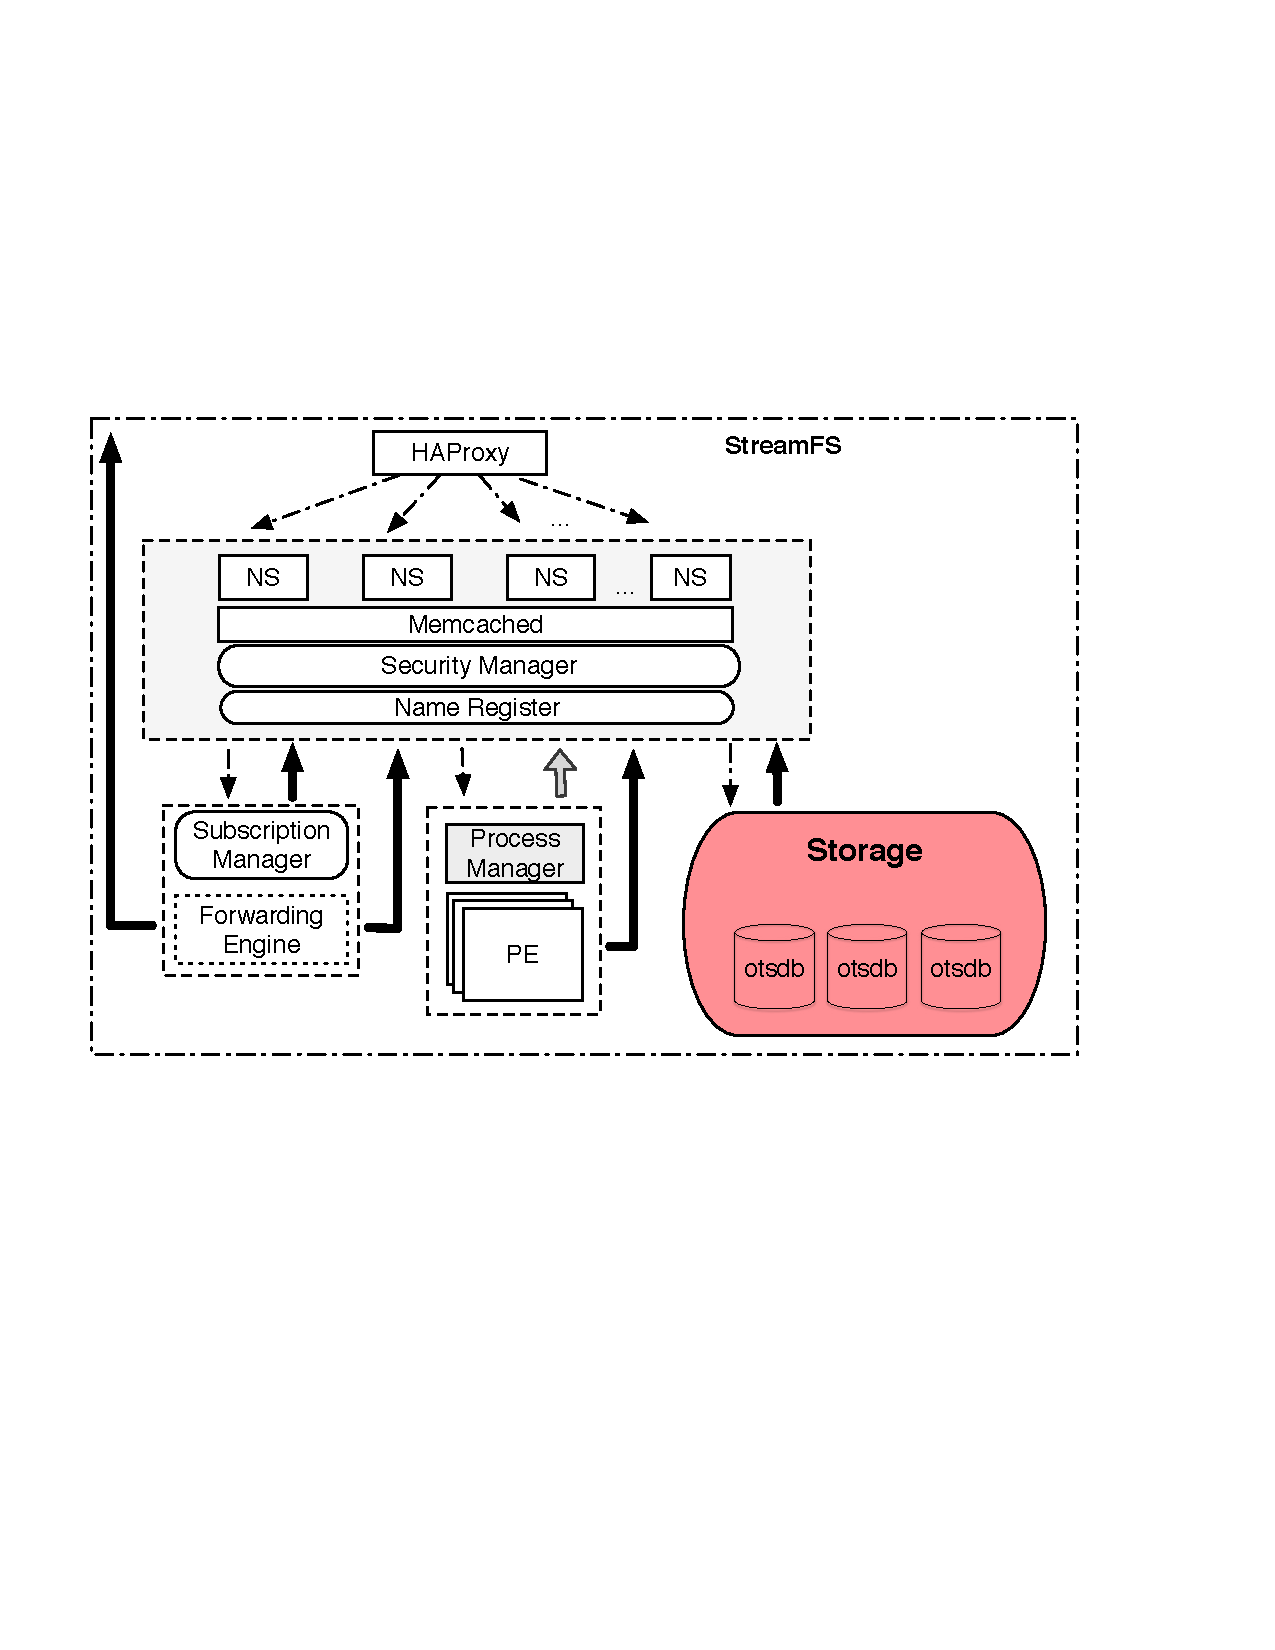
\includegraphics[width=.55\columnwidth]{figs/tsdstore}
\caption{The timeseries data store.  We use OpenTSDB; a timeseries data-store that runs in cluster of
HBase instances.}
\label{fig:tsdb}
\end{figure}

We use OpenTSDB~\cite{opentsdb} as our primary data store. We enable compression  and index on the name and timestamp 
of the feed.  OpenTSDB is a timeseries data store built on HBase~\cite{HBase}.  HBase is designed to scale horizontally for very
large data sets.  OpenTSDB is a good choice because the compression features keep the footprint small/fast while the append-only 
workload requires a scalable solution.
